

\chapter{Theoretical framework}\label{ch:theory}
The current chapter will introduce the theoretical formalism which is used to examine the system of interest in this work. First I will give a brief introduction to the collision model formalism, as it is used to describe the dissipative processes to whom the atomic ensemble is exposed. This model will be used to derive a Lindblad master equation for the system. Proceeding the setup is taken to the thermodynamic limit and the equations of motion for the collective spin operator, which is the sum over all individual spin operators of the atoms, are determined. In a final section I will explain shortly why local pumping is crucial in order to see other long-time states for the collective spin than a featureless fully mixed state.
\section{The collision model}\label{sec:collision_model}
%
Before discussing the exact composition of the system and the involved baths, I will introduce the collision model approach with the example of a generalized Jaynes-Cummings model. For this purpose a two-level atom is supposed to interact with an electromagnetic environment. The electric field is described by a continuous set of modes and the interaction with the atom is modeled in the dipole approximation. The Hamiltonian $H$ for this setup consists of three parts. Two parts describe the free energy of system and field respectively, while the third part implements the interaction between both.
% In this project I will examine a System of N 2-level atoms or spins, described in a collision model framework \cite{ciccarello_quantum_2022,gross_qubit_2018}. The system will be under the influence of several interaction types due to coupling to external baths. The interaction will exhibit laser driving (drive), collective spontaneous emission (SpE), collective dephasing (Dp) and local pumping (pump). The Hamiltonian $H$, describing the interplay of system and bath, is set up in a collision model formalism, which I will introduce in the following.
% % These effects are captured by the collision model Hamiltonian 
% \begin{align}
%     H = H_\text{drive}+H_\text{SpE}+H_\text{Dp}+H_\text{pump}
%     % H &= \frac{\delta}{2}\,J_z+ \omega\,J_x+\alpha\,(J_+a + J_-a^\dagger)+ \beta\,J_z\,(b^\dagger+b)+\xi\,\sum_{i=1}^N\,(\sigma_i^-c_i^\dagger+\sigma_i^+c_i)\\
%     % \text{with}\quad H_S&=\frac{\delta}{2}\,J_z+ \omega\,J_x\\
%     % V_a&=\alpha\,(J_+a- + J_-a^\dagger)\\
%     % V_b&=\beta\,J_z\,(b^\dagger+b)\\
%     % V_c&=\xi\,\sum_{i=1}^N\,(\sigma_i^-c_i^\dagger+\sigma_i^+c_i)\\
%     % J_k &=\half\,\sum_{j=1}^N\sigma_j^k\quad k\in\{x,y,z\}\\
%     % J_\pm&=\half\,\sum_{j=1}^N\sigma_j^\pm\\
%     % \alpha&=\sqrt{\frac{\kappa}{\Delta tN}}\,;\quad \beta=\sqrt{\frac{\gamma}{\Delta t}}\,;\quad \xi=\sqrt{\frac{\Gamma}{4\Delta t}}
% \end{align}
% Before discussing each interaction part, I will first derive the collision model approach exemplarily for the generalized 
% Jaynes-Cummings model, where a continuous set of frequencies is considered. This will be later applied to describe collective spontaneous emission and local pumping. Starting after a dipole approximation has been applied one can write the Hamiltonian of the two level atom in an electromagnetic field as ($\hbar=1$)
\begin{align*}
    H= {\omega_0}\,\ket{e}\bra{e}+2\pi\,\int_{0}^\infty\diff\nu\,\nu\,a^\dagger_\nu a_\nu+ \hat{\boldsymbol{d}}\,\int_{0}^\infty\diff\nu\,\tilde{\alpha}(\nu)\,\boldsymbol{E_0}(\nu)\,(a_\nu+a^\dagger_\nu)
\end{align*}
Here $\ket{e}$ denotes the excited state of the atom. $\omega_0$ is the energy difference of the atomic transition. The energy of the ground state $\ket{g}$ is set to zero. The dipole operator of the transition is noted as $\hat{\mathbf{d}}$, whereas $\mathbf{E_0}(\nu)$ and $\tilde{\alpha}(\nu)$ are the generally written polarization with amplitude and the interaction strength of each mode respectively. The annihilation and creation operators of the electromagnetic frequency modes are labeled by $a_\nu$, $a_\nu^\dagger$. By assuming that only a small number of modes actually contributes to the interaction, one can extend the integral to $-\infty$. One also assumes that the relevant frequency interval is sufficiently narrow that the coupling strength as well as the polarization and amplitude can be approximated as constant therein \cite{ciccarello_quantum_2022,gross_qubit_2018}. Thus it is possible to write the Hamiltonian as
\begin{align*}
    H= {\omega_0}\,\ket{e}\bra{e}+2\pi\,\int_{-\infty}^\infty\diff\nu\,\nu\,a^\dagger_\nu a_\nu+ \tilde{\alpha}\,\boldsymbol{E_0}\,\hat{\boldsymbol{d}}\,\int_{-\infty}^\infty\diff\nu\,(a_\nu+a^\dagger_\nu)
\end{align*}
One can represent the term $\tilde{\alpha}\,\mathbf{E_0}\,\hat{\mathbf{d}}$ in the basis of the atomic ground and excited state $\ket{g}$, $\ket{e}$. Because of the parity properties of the states, all diagonal elements vanish and the representation in the atomic basis takes the form
\begin{align*}
    \tilde{\alpha}\,\hat{\mathbf{d}}\,\mathbf{E_0}&= \tilde{\alpha}'\,\sigma^x=\tilde{\alpha}'\,(\ket{e}\bra{g}+\ket{g}\bra{e})
\end{align*}
with $\tilde{\alpha}'\vcentcolon=\tilde{\alpha}\,\braket{e|\hat{\mathbf{d}}\,\mathbf{E_0}|g}$, what is assumed to be real. Hence the Hamiltonian transforms to
\begin{align*}
    H= {\omega_0}\,\ket{e}\bra{e}+2\pi\,\int_{-\infty}^\infty\diff\nu\,\nu\,a^\dagger_\nu a_\nu+ \tilde{\alpha}'\,\int_{-\infty}^\infty\diff\nu\,\sigma^x\,(a_\nu+a^\dagger_\nu)
\end{align*}
Going to the interaction picture and neglecting counter rotating terms gives rise to the following
\begin{align*}
    H=\tilde{\alpha}'\,\int_{-\infty}^\infty\diff\nu\,(e^{-i\,(2\pi\nu-\omega_0)\, t}\sigma^+a_\nu+e^{i\,(2\pi\nu-\omega_0)\, t}\sigma^-a^\dagger_\nu)\quad,
\end{align*}
$\sigma^+=\ket{e}\bra{g}$ and $\sigma^-=(\sigma^+)^\dagger$ denote the spin ladder operators. This constitutes a generalized Jaynes-Cummings model in the interaction picture. The collision model comes into play, when one introduces combined field operators of the form
\begin{align*}
    a_t\vcentcolon=\int_{-\infty}^{\infty}\diff\nu\,e^{-i\,(2\pi\nu-\omega_0)\, t}a_\nu
\end{align*}
This lets the Hamiltonian read
\begin{align*}
    H= \tilde{\alpha}'\,(\sigma^+a_t+\sigma^-a^\dagger_t)
\end{align*}
The unitary propagation, under which system and bath evolve, can be decomposed into $N$ consecutive propagations of duration $\Delta t$
\begin{align*}
    U(t,t_0)&=\mathcal{T}\left(  \exp(-i\int_{t_0}^t\diff t'\,H(t'))  \right)=U_{N}\cdots U_1\\
    \text{with}\quad U_n&=\mathcal{T}\left( \exp(-i\int_{t_0+(n-1)\,\Delta t}^{t_0+n\,\Delta t}\diff t'\,H(t'))  \right)
\end{align*}
$\mathcal{T}$ is the time ordering operator.
As can be shown \cite{ciccarello_quantum_2022} the propagation can be approximated up to the second order in $\Delta t$ via
\begin{align*}
    U_n \approx 1-i\int_{t_0+(n-1)\,\Delta t}^{t_0+n\,\Delta t}\diff t \,H(t) - \half\,\left(\int_{t_0+(n-1)\,\Delta t}^{t_0+n\,\Delta t}\diff t \,H(t)\right)^2
\end{align*}
After introducing time-bin modes
\begin{align*}
    a_n\vcentcolon&=\frac{1}{\sqrt{\Delta t}}\int_{t_0+(n-1)\,\Delta t}^{t_0+n\,\Delta t}\diff t\,a_t
\end{align*}
and redefining $\alpha=\tilde{\alpha}'/\sqrt{\Delta t}$ this can be written as
\begin{align}\label{eq:approx_time_evolv}
    U_n &\approx 1-i\,H_n \,\Delta t-\half\,H_n^2\,\Delta t^2\notag\\
    \text{with}\quad H_n&=\alpha\,(\sigma_+a_n+\sigma_-a^\dagger_n)
\end{align}
\begin{figure}
    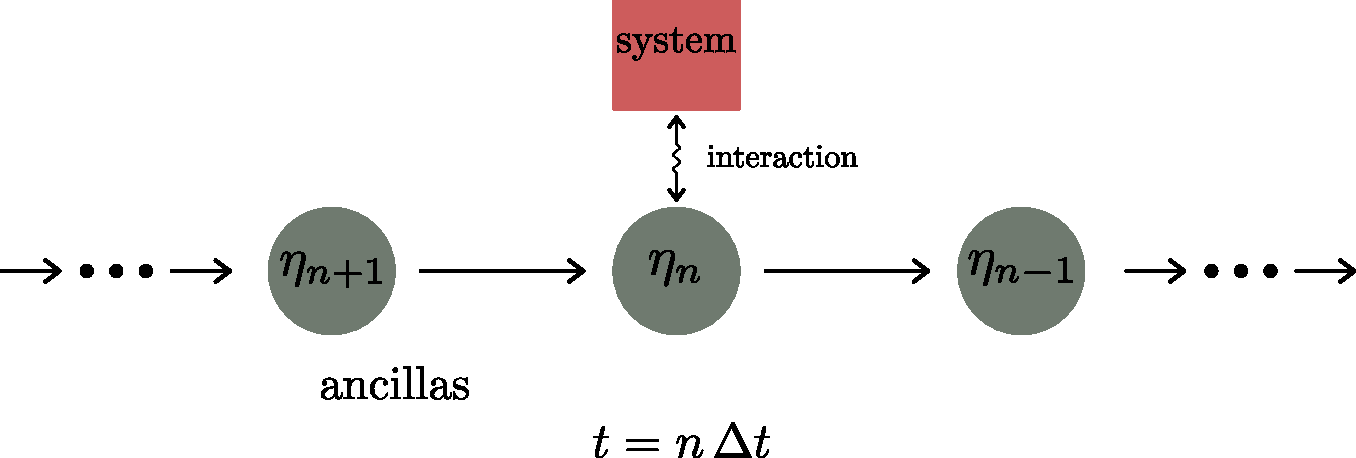
\includegraphics[width=\textwidth]{pictures/cm_scheme.pdf}
    \caption{\textbf{Scheme of system-ancilla interaction.} The consecutive interaction of system and ancillas is depicted. As time moves one the ancillas {\lq move to the right\rq} and interact one at a time with the system. When the time step is taken to zero, the interaction becomes continuous and models the bath as not sustainedly influenced by the system, similar to the Markov approximation.}\label{fig:cm_scheme}
\end{figure}
The evolution of the system factorizes into consecutive interactions described by the Hamiltonian $H_n$, as illustrated in \figref{fig:cm_scheme}. Those interactions can be interpreted as $N$ independent bath segments, called in the following ancillas, interacting separately with the system, when the following property holds. At each such interaction the state of the bath is completely uncorrelated  to and not influenced by what has happened during the previous interactions - or at least so up to a sufficient degree. In this case the main criteria for a description through the collision model are met, which are \cite{ciccarello_quantum_2022}: 
\begin{itemize}
    \item ancillas do not interact with each other 
    \item ancillas are initially uncorrelated 
    \item each ancilla collides with the system only once 
\end{itemize}
Notice that those ideas are also related to the Born Markov approximations. The assumption of independent consecutive interactions leans on the assumption of a correlation time of the bath, which is much smaller than the one of the system. Note, that $[a_n,a^\dagger_{n'}]=\delta_{n,n'}$ holds, which strengthens the notion of independent modes.\\\\%, and therefore the modes of different $n$ do not depend on each other, which is important for being able to describe the system via a collision model with collisions with ancillas $n$.
One has to take into account that for the system, which is considered in this project, local as well as collective interaction is chosen. This also has implications for the correlations between system and bath.
In order for an interaction, e.g. spontaneous emission, to be collective one has to realize a field that couples to all atoms at once. The temporal and spatial correlation of the field have to reach far enough such that the time between emissions as well as the distance between the atoms is smaller than correlation time and length. \\Local interaction with the bath on the other hand demands that the interaction of one atom with the bath has no influence on the interaction of another atom with the bath. This demands sufficiently small spatial and temporal correlations. Hence the physical implementation of such a system requires experimental tact \cite{diehl_quantum_2008,shaw_multi-ensemble_2024}.\\\\% It is often realized in optical cavities \cite{shaw_multi-ensemble_2024}.\\\\%Hence with those two electromagnetic environments one has to find  a sweet spot of the coupling implementations, where both requirements for the different interactions can be satisfied, if one wants to implement a physical system of such character.\\\\
\section{Composition of the system}\label{sec:composition_of_model}
In this project I will examine a system of N non-interacting 2-level atoms or spins. They will be under the influence of several interaction types due to coupling to external baths. The interaction will exhibit laser driving (drive), collective spontaneous emission (SpE), collective dephasing (Dp) and local pumping (pump). These effects are captured by the collision model Hamiltonian 
\begin{align}
    H = H_\text{drive}+H_\text{SpE}+H_\text{Dp}+H_\text{pump}
    % H &= \frac{\delta}{2}\,J_z+ \omega\,J_x+\alpha\,(J_+a + J_-a^\dagger)+ \beta\,J_z\,(b^\dagger+b)+\xi\,\sum_{i=1}^N\,(\sigma_i^-c_i^\dagger+\sigma_i^+c_i)\\
    % \text{with}\quad H_S&=\frac{\delta}{2}\,J_z+ \omega\,J_x\\
    % V_a&=\alpha\,(J_+a- + J_-a^\dagger)\\
    % V_b&=\beta\,J_z\,(b^\dagger+b)\\
    % V_c&=\xi\,\sum_{i=1}^N\,(\sigma_i^-c_i^\dagger+\sigma_i^+c_i)\\
    % J_k &=\half\,\sum_{j=1}^N\sigma_j^k\quad k\in\{x,y,z\}\\
    % J_\pm&=\half\,\sum_{j=1}^N\sigma_j^\pm\\
    % \alpha&=\sqrt{\frac{\kappa}{\Delta tN}}\,;\quad \beta=\sqrt{\frac{\gamma}{\Delta t}}\,;\quad \xi=\sqrt{\frac{\Gamma}{4\Delta t}}
\end{align}
This Hamiltonian models the dynamics of system and ancilla. To keep the notation simpler, the $n$, which indicates the time step, i.e. the current ancilla, is omitted, as will be done throughout the section. I will now discuss the origin and form, of how each interaction process is modeled.
Collective spontaneous emission results from a dipole interaction of the atom with an electromagnetic field. It constitutes the generalized Jaynes-Cummings model mentioned in the previous section. The property that determines the explicit effect of the interaction is the state of the field, i.e. the state of the ancilla.\\
For the description of emission one can choose the initial state of each ancilla as the vacuum state, as for sufficiently low emission rate, such an ancilla only triggers emissions. According to the derivation in \secref{sec:collision_model} the collective spontaneous emission can be build into the Hamiltonian with the following form.
\begin{align*}
    H_\text{SpE}&=\alpha\,(J_+a + J_-a^\dagger)
\end{align*}
$J_\pm$ are the collective spin lowering and rising operators, i.e. the sum of the ladder operators of each atom 
\begin{align*}
    J_\pm=\sum_{i=1}^N\sigma^\pm_i
\end{align*}
and $a$, $a^\dagger$ are the bosonic field operators of the collision model, $\alpha$ is the effective coupling constant.\\\\


The treatment of local pumping requires more care. %the initial ancilla states to be in an excited state.
Experimentally it can be implemented by applying an excitation scheme that uses different energy levels during the process \cite{meiser_prospects_2009}. One can simplistically imagine a scheme similar to the realization of occupation inversion in laser physics. The atom is excited by the pumping laser into a specific higher energy level which relaxes quickly into the $\ket{e}$-state of the model. The fact that the pumping comes in the final step from a higher level of the same atom causes the process to be local.

The mathematical description has to prevent an exited atom from decaying through this system-bath interaction channel. This is achieved through the short interaction time, i.e. the continuous time limit, and the modeling of the bath as two level system. Choosing the initial ancilla state to be the excited one of the bath leads to the wanted pumping. The effective collision model Hamiltonian reads 
\begin{align*}
    H_\text{pump}&=\xi\,\sum_{i=1}^N\,(\sigma_i^-c_i^\dagger+\sigma_i^+c_i)
\end{align*}
with two level annihilation and excitation operators $c_i$, $c_i^\dagger$, which are separately connected to each atom. Collective dephasing is also implemented in a collision model form for this project. %But it needs a different field atom interaction, which I don't want to derive here. 
Experimentally dephasing can be simulated through spin-dependent kick operations\cite{sun_quantum_2024}. The theoretical description takes the form % It can be introduced through a classical field, which has minima at the atomic positions, but has for all atoms the same values. Then the deviation of the atom from the position of the minimum can be described by a bosonic mode. The justification of a collision model approach has to be made by saying, the atom, if dislocated, relaxes back to the minimum in way shorter time scales than the ones the dynamics of the system is described at. How this relaxation is achieved, I don't know.
\begin{align*}
    H_\text{Dp}&=\beta\,J_z\,(b^\dagger+b)\quad,
\end{align*}
again with a bosonic field mode $b$, $b^\dagger$ in the collision model picture. Completing the introduction of the fully quantum mechanically described coupling, I set the so far introduced coupling constants to the form
\begin{align}
    \alpha&=\sqrt{\frac{\kappa}{\Delta tN}}\,;\quad \beta=\sqrt{\frac{\gamma}{\Delta t}}\,;\quad \xi=\sqrt{\frac{\Gamma}{4\Delta t}}
\end{align}
This choice becomes helpful in the derivation of the Lindblad equation.\\\\
The last feature, that has not been addressed yet, is the laser driving. This will be treated semiclassically, which is possible if the field is strong enough, so that the behavior of the atoms has no influence on the state of this light field. The corresponding term in the Hamiltonian can be derived by starting with the single mode light-atom interaction in the dipole approximation, where the field operators are replaced by the amplitude of the large coherent state, according to the negligible influence of the dynamics of the system on the electromagnetic field. 
% The operators acting on the system are the pauli spin matrices $\sigma^{x,y,z}$. I will go through the terms, where I will label them and explain their derivation. $\delta$ labels the detuning of a laser driving coupled with the parameter $\omega$. The responsible field is treated classically, which is possible if the field is strong enough, so that the behavior of the atoms has no influence on the state of this light field. The term can be derived by starting with the light atom interaction in the dipole approximation.
\begin{align*}
    H_\text{drive} = \omega_0\,\ket{e}\bra{e}+ \varepsilon\,\hat{\mathbf{d}}\,\mathbf{E_0}\,\cos(\omega_Lt)\quad,
\end{align*} 
$\varepsilon$ is the coupling strength. As the laser field is not described quantum mechanically, it has to be introduced already as time dependent in the Schrödinger picture. After representing the dipole operator in the atomic basis as was done earlier, I define $\varepsilon\,\hat{\mathbf{d}}\,\mathbf{E_0}=\vcentcolon2\omega\,\sigma^x$. Consequently the interaction with the driving laser takes the form
\begin{align*}
    H_\text{drive} = \omega_0\,\ket{e}\bra{e}+ 2\omega\,\sigma^x\,\cos(\omega_Lt)\quad,
\end{align*}
In order to arrive at the final form, one has to perform a gauge transformation. This gauge transformation has to be chosen with respect to the whole Hamiltonian. I demonstrate the transformation on the reduced Hamiltonian which only includes laser driving and one spontaneous emission mode.
\begin{align*}
    \tilde{H} = \omega_0\,\ket{e}\bra{e}+ 2\omega\,\sigma^x\,\cos(\omega_Lt)+\omega\,a^\dagger_\omega a_\omega+ \tilde{\alpha}\,\boldsymbol{E_0}\,\hat{\boldsymbol{d}}\,(a_\omega+a^\dagger_\omega)
\end{align*}
In this context one chooses the unitary transformation 
\begin{align*}
    U&=\exp\left(i\omega_L t\,\ket{e}\bra{e}+i\omega t\,a_\omega^\dagger a_\omega\right)\\
    &=\left[ \exp(i\omega t)\,\ket{e}\bra{e}+\ket{g}\bra{g} \right]\otimes \exp\left( i\omega t\,a_\omega^\dagger a_\omega \right)
\end{align*}
The Hamiltonian is affected in the following way by the transformation
\begin{align*}
    \tilde{H}\rightarrow \,&U\tilde{H}U^\dagger+i\,(\frac{\diff}{\diff t}\,U)\,U^\dagger\\
    &=\omega_0\,\ket{e}\bra{e}-\omega_L\,\ket{e}\bra{e} + 2\omega\,\cos(\omega_L t)\,\{e^{i\omega_L t} \ket{e}\bra{g}+e^{-i\omega_L t}\ket{g}\bra{e}\}\\
    &+\tilde{\alpha}'\,\{e^{i\omega_L t} \ket{e}\bra{g}+e^{-i\omega_L t}\ket{g}\bra{e}\}\,\{ e^{-i\omega t} \,a_\omega+e^{i\omega t}\,a_\omega^\dagger  \}-\omega\,a^\dagger_\omega a_\omega\\\\
    =\,&(\omega_0-\omega_L)\,\ket{e}\bra{e}+\omega\,\sigma_x+\tilde{\alpha}'\,\left( e^{-i\,(\omega-\omega_L)\, t}\,\sigma^+\,a_\omega+e^{i\,(\omega-\omega_L)\, t}\,\sigma^-\,a^\dagger_\omega \right)
\end{align*}
Between the second to third step the terms containing counter rotating exponentials have been neglected. By resetting the zero energy point to the middle of the atomic states and defining the detuning $\delta=\omega_0-\omega_L$ the Hamiltonian can be written as
\begin{align*}
    \tilde{H} = \frac{\delta}{2}\,\sigma^z+ \omega\,\sigma^x+\tilde{\alpha}'\,\left( e^{-i\,(\omega-\omega_L)\, t}\,\sigma^+\,a_\omega+e^{i\,(\omega-\omega_L)\, t}\,\sigma^-\,a^\dagger_\omega \right)
\end{align*}
This can be easily generalized to $N$ atoms.
In summary, when combining the effect of the laser driving with the different interaction mechanisms from the external baths, the full Hamiltonian arises, which describes the dynamics of system and ancillas.
\begin{align}\label{eq:full_Ham}
    H &= \frac{\delta}{2}\,J_z+ \omega\,J_x+\alpha\,(J_+a + J_-a^\dagger)+ \beta\,J_z\,(b^\dagger+b)+\xi\,\sum_{i=1}^N\,(\sigma_i^-c_i^\dagger+\sigma_i^+c_i)
\end{align}



\section{Derivation of the Lindblad equation}%[Lindblad equation]
The master equation is derived by evolving the density matrices of system and ancillas during their interplay. Because of the assumed short time of interaction the previously derived propagation operator up to second order in the interaction time interval is used (\ref{eq:approx_time_evolv}).
\begin{align}
    U_n &\approx 1-i\,H_n \,\Delta t-\half\,H_n^2\,\Delta t^2
\end{align}
Here the labeling of the ancillas (by the index $n$) is reintroduced.
The Hamiltonian $H_n$ (\refeq{eq:full_Ham}) is decomposed in a term that solely effects the system and one that describes the interaction with the baths.
\begin{align}\label{eq:Ham_split}
    H_n &= H_n^S + V_n\notag\\
    H_n^S&=\frac{\delta}{2}\,J_z+\omega\,J_x\notag\\
    V_n&= \alpha\,(J_+a_n + J_-a_n^\dagger)+ \beta\,J_z\,(b_n^\dagger+b_n)+\xi\,\sum_{i=1}^N\,(\sigma_{i}^-c_{n,i}^\dagger+\sigma_i^+c_{n,i})
\end{align}
The density matrix $\chi$ of the composite system ($\rho$) and ancilla ($\eta_n$) is , as discussed, assumed to be initially uncorrelated $\chi_n=\rho_n\otimes\eta_n$, where $\rho_n$ is the density matrix of the system at the beginning of the $n$th $\Delta t$-interval. At the end of the $n$th system-ancilla interaction, the state of the density matrix has evolved to
\begin{align*}
    \chi_n\left((n+1)\,\Delta t\right)&=U_n\chi_nU_n^\dagger
\end{align*}
Here $ \chi_n((n+1)\,\Delta t)$ represents the state of system and ancilla at the end of the interaction, which is in general mixed.
If one now plugs in the approximate form of the propagation $U_n$, the following expression is found
\begin{align*}
    \chi_n\left((n+1)\,\Delta t\right)-\chi_n&=-i\,[H_n,\chi_n]\,\Delta t+H_n\,\chi_n\,H_n\,\Delta t^2+\half\,[H_n^2,\chi]_+\,\Delta t^2
\end{align*}
where $[\cdot,\cdot]_+$ is the anticommutation relation. The terms quadratic in $H_n^S$ can be neglected, as is explained in \cite{ciccarello_quantum_2022}. The equation of motion becomes thus
\begin{align}
    \chi_n\left((n+1)\,\Delta t\right)-\chi_n=\Delta\chi_n\vcentcolon=-i\,[H_n,\chi_n]\,\Delta t+V_n\,\chi_n\,V_n\,\Delta t^2+\half\,[V_n^2,\chi]_+\,\Delta t^2\label{eq:pre_lindblad}
\end{align}
Tracing out the baths at this point gives the density matrix of the system at the beginning of the subsequent time step. 
\begin{align*}
    \rho_{n+1}=\rho_n\left((n+1)\,\Delta t\right)&=\Trb{\chi_n\left((n+1)\,\Delta t\right)}\\
    \Delta\rho_n&=\rho_{n+1}-\rho_n
\end{align*}
Performing this operation to both sites of \eqref{eq:pre_lindblad} leads to the Lindblad equation for the density matrix of the system. In the following I will drop the subscript $n$. For better orientation I split the master equation into different segments.
\begin{align*}
    \frac{\Delta\rho}{\Delta t}=\left(L_\text{drive}+L_\text{SpE}+L_\text{Dp}+L_\text{pump}\right)(\rho)
\end{align*}
As the the expectation values of the interaction operators on the bath side vanish in our case, the first term becomes
\begin{align*}
    L_\text{drive}(\rho)=-i\,[H_S,\rho]
\end{align*}
The part associated with collective spontaneous emission takes the form
\begin{align*}
    L_\text{SpE}(\rho) &= \alpha^2\,\Trb{H_\text{SpE}\,\chi \,H_\text{SpE}-\half\,[H_\text{SpE}^2,\chi]_+}\,\Delta t\\
    &= \frac{\kappa}{N}\,J_-\rho J_+\,\Trb{a\,a^\dagger\eta_\text{SpE}}-\half\,\frac{\kappa}{N}\,[J_+J_-,\rho]_+\,\Trb{[a\,a^\dagger,\eta_\text{SpE}]_+}\\
    &=\frac{\kappa}{N}\,(J_-\rho J_+-\half\,[J_+J_-,\rho]_+)\\
    \text{for}\quad\eta_\text{SpE}&=\ket{\text{vac}}\mathrel{\substack{\,\\\,\\ \text{SpE}}}\bra{\text{vac}}
\end{align*}
From the start I excluded the vanishing terms $\Trb{(a^\dagger a^\dagger+a\,a+a^\dagger a)\cdot\eta}$. With the choice $\eta_\text{Dp}=\ket{\text{vac}}\mathrel{\substack{\,\\\,\\ \text{Dp}}}\bra{\text{vac}}$ and $\eta^\text{pump}_i=\ket{1}\mathrel{\substack{\text{pump}\\\,\\ i}}\bra{1}$ the terms for dephasing and pumping arise analogously
\begin{align}
    L_\text{Dp}(\rho)%&= \beta^2\,J_z\rho J_z\, \Trb{b\,b^\dagger\eta_b}\,\Delta t-\beta^2\,\half\,[J_z^2,\rho]_+\,\Trb{[b\,b^\dagger,\eta_b]_+}\,\Delta t\\
    &=\gamma\,J_z\rho J_z-\half\,\gamma\,[J_z^2,\rho]_+\\
    % \eta_b&=\ket{\text{vac}}_b\bra{\text{vac}}\\
    L_\text{pump}(\rho)%&= \xi^2\,\sum_i\sigma_i^-\rho \sigma_i^+\, \Trb{c_i^\dagger c_i\eta^c_i}\,\Delta t-\xi^2\,\half\,\sum_i\,[\sigma_i^-\sigma_i^+,\rho]_+\,\Trb{[c_i^\dagger c_i,\eta^c_i]_+}\,\Delta t\\
    &=\frac{\Gamma}{4}\,\left(\sum_i\sigma_i^+\rho \sigma_i^--\half\,\sum_i\,[\sigma_i^-\sigma_i^+,\rho]_+\right)\label{eq:pumping_Lindblad_op}
    % \eta^c_i&=\ket{1}^c_i\bra{1}
\end{align}
%In order to reach at expression \ref{eq:pumping_Lindblad_op} one has to respect a suitable excitation scheme, as discussed earlier. 
In the limit of very short interaction times with each ancilla $\Delta t\rightarrow0$, the density matrix dynamics of the system approach a continuous time propagation. The time evolution of the expectation value of an observable $O_S$ can thus be determined via 
\begin{align}
    \dt \braket{O_S}=\Trs{O_S\,\dt\rho}&=\Trs{O_S\,\left(L_\text{drive}(\rho)+L_\text{SpE}(\rho)+L_\text{Dp}(\rho)+L_\text{pump}(\rho)\right)}\notag\\
    &=\vcentcolon \mathcal{L}_\text{drive}(O_S)+\mathcal{L}_\text{SpE}(O_S)+\mathcal{L}_\text{Dp}(O_S)+\mathcal{L}_\text{pump}(O_S)
\end{align}

\section{Equation of motion for the collective spin}\label{sec:mean_field_eq}%[mean field equations]
Starting from the Lindblad equation one can derive the equations of motion for the collective spin of the system. I will again divide the derivation of the full dynamics into the contributions of the different couplings. The effect of the laser driving constitutes 
\begin{align*}
    \mathcal{L}_\text{drive}(J_z)&=\omega\,\braket{J_y}\\
    \mathcal{L}_\text{drive}(J_\pm)&=-i\,\left(\mp\frac{\delta}{2}\, \braket{J_\pm} \pm \omega\, \braket{J_z}\right)
\end{align*}
The other interaction types can be found to contribute in the following way to equations of motion
\begin{align*}
    \mathcal{L}_\text{SpE}(J_z)=-\frac{\kappa}{N}\,\Trs{J_+ J_- \rho},\quad
    \mathcal{L}_\text{SpE}(J_+)=\frac{\kappa}{N}\,\Trs{J_+ J_z \rho},\quad
    \mathcal{L}_\text{SpE}(J_-)=\frac{\kappa}{N}\,\Trs{J_z J_- \rho}
\end{align*}
\begin{align}
    \mathcal{L}_\text{Dp}(J_z)=0,\quad
    \mathcal{L}_\text{Dp}(J_\pm)=-\half\,\gamma\,\Trs{J_\pm\rho}
\end{align}
\begin{align*}
    \mathcal{L}_\text{pump}(J_z)=\half\,N\,\Gamma-\Gamma\,\braket{J_z},\quad
    \mathcal{L}_\text{pump}(J_-)=-\frac{\Gamma}{2}\,\sum_{k=1}^N\Trs{\sigma_k^-\rho},\quad
    \mathcal{L}_\text{pump}(J_+)=-\frac{\Gamma}{2}\,\sum_{k=1}^N\Trs{\sigma_k^+\rho}
\end{align*}
Detailed computations of those expressions have been shifted to the \appref{appendix:eqm_derv}. Hence joining all the different contributions one arrives at the equations of motion
\begin{align}
    \dt \braket{J_+}&=\,i\,\frac{\delta}{2}\,\braket{J_+}-i\,\omega\,\braket{J_z}-\half\,(\gamma+\Gamma)\,\braket{J_+}+\frac{\kappa}{N}\,\braket{J_+ J_z}\notag\\
    \dt \braket{J_-}&=-i\,\frac{\delta}{2}\,\braket{J_-}+i\,\omega\,\braket{J_z}-\half\,(\gamma+\Gamma)\,\braket{J_-}+\frac{\kappa}{N}\,\braket{J_z J_-}\notag\\
    &=-i\,\frac{\delta}{2}\,\braket{J_-}+i\,\omega\,\braket{J_z}-\half\,(\gamma+\Gamma)\,\braket{J_-}+\frac{\kappa}{N}\,\braket{J_- J_z}-\frac{\kappa}{N}\,\braket{J_-}\notag\\
    \dt \braket{J_z}&=\omega\,\braket{J_y} - \frac{\kappa}{N}\,\braket{J_+ J_-}+\half\,N\,\Gamma-\Gamma\,\braket{J_z}
\end{align}
The representation can be transformed from the ladder operators back to the spin components.
\begin{align*}
    \dt\,\braket{J_x}=\half\,\left(\dt \braket{J_+}+\dt \braket{J_-}\right)&=-\frac{\delta}{2}\,\braket{J_y}-\half\,(\gamma+\Gamma)\,\braket{J_x}+\frac{\kappa}{N}\,\braket{J_xJ_z}-\frac{\kappa}{2N}\,\braket{J_-}\\
    \dt\,\braket{J_y}=-i\,\half\,\left(\dt \braket{J_+}-\dt \braket{J_-}\right)&=\frac{\delta}{2}\,\braket{J_x}-\omega\,\braket{J_z}-\half\,(\gamma+\Gamma)\,\braket{J_y}+\frac{\kappa}{N}\,\braket{J_yJ_z}-i\,\frac{\kappa}{2N}\,\braket{J_-}\\
    \dt \braket{J_z}&=\omega\,\braket{J_y} - \frac{\kappa}{N}\,\braket{J_x^2+J_y^2} -\frac{\kappa}{N}\,\braket{J_z}+\half\,N\,\Gamma-\Gamma\,\braket{J_z}
\end{align*}
The aim of this project is to analyze the system in the thermodynamic limit. In this limit the mean-field treatment is correct, i.e. for two operators $A$ and $B$ the joined expectation value becomes $\braket{A\,B}=\braket{A}\,\braket{B}$. For the transformation of the dynamical equations into mean-field equations of motion I define the observable of the system as expectation value of the spin components $m_\alpha=\braket{J_\alpha}/N$. As a consequence of the thermodynamic limit terms proportional to $\braket{J_\alpha}/N^2\rightarrow0$ vanish and the mean field equations of motion thus read
\begin{align}
    \dt m_x &= -\frac{\delta}{2}\,m_y-\half\,(\gamma+\Gamma)\,m_x+\kappa\,m_x m_z\notag\\
    \dt m_y &= \frac{\delta}{2}\,m_x-\omega\,m_z-\half\,(\gamma+\Gamma)\,m_y+\kappa\,m_y m_z\notag\\
    \dt m_z &= \omega\,m_y - \kappa\,(m_x^2+m_y^2)+\half\Gamma-\Gamma\,m_z\label{eq:mean_field}
\end{align}
They constitute a coupled set of three non-linear differential equations of first order.
\section{The importance of local pumping}
The emphasis of this project will be the analysis of the long-time states, the systems occupies in the thermodynamic limit. For the occurrence of non trivial long-time behavior, however, local pumping  is crucial. In its absence the system decays to the fully mixed state. This can be recognized by taking a look at the properties of the total spin.
\begin{align}\label{eq:total_momentum_decay}
    m^2\vcentcolon&=m_x^2+m_y^2+m_z^2\notag\\
    \Rightarrow\quad\dt m^2&=2\,\left( m_x\,\dt m_x +m_y\,\dt m_y +m_z\,\dt m_z \right)\notag\\
    &=-\vec{m}^t\,\left( \begin{array}{ccc}
        \Gamma+\gamma & 0&0  \\
        0& \Gamma+\gamma & 0\\
        0&0&2\,\Gamma
   \end{array}\right)\,\vec{m}+\Gamma\,m_z\notag\\
   &=-\left(  (\Gamma+\gamma)\,(m_x^2+m_y^2)+2\,\Gamma\,m_z^2-\Gamma\,m_z \right)
\end{align}
Because without pumping $\Gamma=0$, the derivative of $m^2$ reduces to the matrix scalar product, the derivative is always negative for positive definite matrices.  In \appref{appendix:msq_calc} it is shown that in our case the positive semi-definiteness of the matrix is sufficient for the system to always decay to the fully mixed state. From \eqref{eq:total_momentum_decay} can also be told that laser driving, detuning and collective spontaneous emission have no direct influence on the total spin modulus.
